\section{Topologies} 

  The first thing to define is a topology. 

  \begin{definition}[Topology]
    Let $X$ be a set and $\T$ be a family of subsets of $X$. Then $\T$ is a \textbf{topology} on $X$\footnote{I will use script letters to denote topologies and capital letters to denote sets.} if it satisfies the following properties. 
    \begin{enumerate}
      \item \textit{Contains Empty and Whole Set}: 
      \begin{equation}
        \emptyset, X \in \T
      \end{equation}

      \item \textit{Closure Under Union}. If $\{U_\alpha\}_{\alpha \in A}$ is a class of sets in $\T$, then 
      \begin{equation}
        \bigcup_{\alpha \in A} U_\alpha \in \T
      \end{equation}

      \item \textit{Closure Under Finite Intersection}: If $U_1, \ldots, U_n$ is a finite class\footnote{Note that we restrict property 3 to be a \textit{finite} intersection because it turns out that the finiteness of intersection allows us to prove many nice properties about topologies, which we will mention later. Another reason is that if we remove this finite restriction, the open ball topology on $\mathbb{R}$ would imply that $\cap_{i = 1}^{\infty} ( - 1/i, +1/i ) = 0$ is an open set $\implies$ all points are open sets too, which is generally not what we want in analysis. 
      } of sets in $\T$, then 
      \begin{equation}
       \bigcap_{i=1}^{n} U_i \in \T
      \end{equation}
    \end{enumerate}
    A \textbf{topological space} is denoted $(X, \T)$. 
  \end{definition}

  For the sake of giving at least one nontrivial example, here is an example of a finite topology. 

  \begin{example}[Topologies of a Set of Cardinality 3]
    There are a total of 29 topologies that we can construct on $\{1, 2, 3\}$. Two such examples are 
    \begin{enumerate}
      \item $\{\emptyset, \{1, 2\}, \{1, 2, 3\}\}$ 
      \item $\{\emptyset, \{3\}, \{2, 3\}, \{1, 2, 3\}\}$
    \end{enumerate}
  \end{example} 

  When we define a new topology, we must first prove that they are topologies, and so these definitions are really theorems. However, I will introduce them as definitions and reserve the theorem environment for actual theorems. 

  \begin{definition}[Discrete, Indiscrete Topologies]
    Given a set $X$, 
    \begin{enumerate}
      \item $2^X$ is a topology, called the \textbf{discrete topology}. 
      \item $\{\emptyset, X \}$ is a topology, called the \textbf{indiscrete topology}. 
    \end{enumerate}
  \end{definition}
  \begin{proof}
    Listed. 
    \begin{enumerate}
      \item The first property is trivially proven. From the theorems of set theory, $U_\alpha \subset X \implies \cup U_\alpha \subset X \implies \cup U_\alpha \in 2^X$. Finally the same logic holds for intersection as well. 
      \item The first property is trivially proven. We can check for the 4 combinations of unions and intersections and see that they all result in either $\emptyset$ or $X$. 
    \end{enumerate}
  \end{proof}

  Here is our first nontrivial example of a topology. It's nice that it can be directly constructed given any set, with no additional structure. 

  \begin{definition}[Cofinite Topology]
    Given a set $X$, the set of all subsets $U$, satisfying the property that $X \setminus U$ is finite, is a topology, called the \textbf{cofinite topology} or the \textbf{finite complement topology}.\footnote{While this definition may seem a bit arbitrary, this is very similar to the Zariski topology, which is used in algebraic topology.} 
  \end{definition}
  \begin{proof}
    Let us denote this set $\T_c$. 
    \begin{enumerate}
      \item By definition $\emptyset \in \T_c$. It is clear that $X \setminus X = \emptyset$ has cardinality $0$, and therefore is in $\T_c$. 

      \item Let $\{U_\alpha\}_{\alpha \in I} \in \mathcal{T}_c$ by a collection of open sets of $X$. Then by deMorgan's laws, 
      \begin{equation}
        X \setminus \bigcup_{\alpha \in I} U_{\alpha} = \bigcap_{\alpha \in I} (X \setminus U_\alpha)
      \end{equation}
      $X \setminus U_\alpha$ is countable for all $\alpha \in I$, so let us fix some $\alpha^\prime$. Then 
      \begin{equation}
        \bigcap_{\alpha \in I} (X \setminus U_\alpha) \subset U_{\alpha^\prime} \implies \bigg| \bigcap_{\alpha \in I} (X \setminus U_\alpha) \bigg| \leq \big| U_{\alpha^\prime} \big| 
      \end{equation}
      and so the intersection is also countable. 

      \item Let $\{U_i\}_{i=1}^n$ by a finite collection of open sets of $X$. Then by deMorgan's laws, 
      \begin{equation}
        X \setminus \bigcap_{i=1}^n U_i = \bigcup_{i=1}^n (X \setminus U_i)
      \end{equation}
      Since $U_i$ are open, $X \setminus U_i$ are countable, and since the finite union of countable sets are countable, the RHS is countable, which implies the LHS is countable and so $\cap_{i=1}^n U_i$ is open as well. 
    \end{enumerate}
  \end{proof} 

  Slightly modifying the definition does not result in a topology. 

  \begin{example}[Countable Complement is Not A Topology]
    Given a set $X$, consider the collection 
    \begin{equation}
      \T_\infty \coloneqq \{U \subset X \mid X \setminus U \text{ is infinite or empty or all of }X \}
    \end{equation}
    This is not a topology. Let us take $X = \mathbb{R}$, and look at the sets $\mathbb{Z}_{\geq 0}, \mathbb{Z}_{\leq 0}$ consisting of all the non-negative and non-positive integers. They are both infinite, and so $\mathbb{R} \setminus \mathbb{Z}_{\geq 0}$ and $\mathbb{R} \setminus \mathbb{Z}_{\leq 0}$ are in $\mathcal{T}_\infty$. Consider their union. 
    \begin{equation}
      (\mathbb{R} \setminus \mathbb{Z}_{\geq 0}) \cup (\mathbb{R} \setminus \mathbb{Z}_{\leq 0}) = \mathbb{R} \setminus (\mathbb{Z}_{\geq 0} \cap \mathbb{Z}_{\leq 0}) = \mathbb{R} \setminus \{0\}
    \end{equation}
    But $\mathbb{R} \setminus (\mathbb{R} \setminus \{0\}) = \{0\}$, and so $\mathbb{R} \setminus \{0\}$ is not open. Therefore $\mathcal{T}_c$ doesn't satisfy the definition of a topology. 
  \end{example}


  \begin{definition}[Finer, Coarser Topologies]
    Suppose that $\T$ and $\T^\prime$ are two topologies on a given set $X$. If $\T \subset \T^\prime$, we say that $\T^\prime$ is \textbf{finer} than $\T$, or equivalently, we say that $\T$ is \textbf{coarser} than $\T^\prime$. 
  \end{definition}

  We can think of the topology of a set $X$ as a truck full of gravel as the open sets. If the gravel is smashed into smaller, finer pieces, then the amount of stuff that we can make from the finer gravel increases, which corresponds to a bigger topology. Clearly, the indiscrete topology is the coarsest topology and the discrete topology is the finest. 

  \begin{theorem}[Intersection of Topologies]
    Given a family of topologies $\{\T\}_{\alpha \in A}$, the set 
    \begin{equation}
      \T = \bigcap_{\alpha \in A} \T_\alpha
    \end{equation}
    is a topology. 
  \end{theorem}

  \begin{corollary}[Unique Coarsest and Finest Topology]
    Given a family of topologies $\{\T\}_{\alpha \in A}$, there exists 
    \begin{enumerate}
      \item a unique smallest topology on $X$ containing all the collections $\T_\alpha$. 
      \item a unique largest topology on $X$ contained in each $\T_\alpha$. 
    \end{enumerate}
  \end{corollary} 

  \begin{example}
    Let $X = \{a, b, c\}$, and let 
    \begin{align}
      \T_1 & = \{\emptyset, X, \{a\}, \{a, b\}\} \\
      \T_2 & = \{\emptyset, X, \{a\}, \{b, c\}\}
    \end{align}
    We claim that the 
    \begin{enumerate}
      \item smallest topology containing $\T_1, \T_2$ is 
      \begin{equation}
        \T_{1 \cup 2} = \{\emptyset, X \{a\}, \{b\}, \{a, b\}, \{b, c\}\}
      \end{equation} 
      Note that this is not simply the union of topologies. The union wouldn't have $\{b\}$, making it not a topology. 

      \item largest topology contained in $\T_1, \T_2$ is 
      \begin{equation}
        \T_{1 \cap 2} = \{\emptyset, X, \{a\}\}
      \end{equation}
      Note that this is simply the intersection of the two topologies. 
    \end{enumerate}
  \end{example}

\subsection{Open Sets}

  This leads to the most general definition of an open set. Note that an open set doesn't really mean anything without talking about with respect to its topology. 

  \begin{definition}[Open Set]
    The elements of $\T$ are called \textbf{open sets} in $X$.\footnote{As implied from the definition of a topology, the arbitrary union and finite intersection of any number of open sets is an open set.} 
    \begin{enumerate}
      \item An open set $U$ which contains a point $x$ is called an \textbf{open neighborhood} of $x$, denoted $U_x$. 
      \item Given an open neighborhood $U_x$ of $x$, the set $U_x \setminus \{x\}$ is called the \textbf{punctured open neighborhood} of $x$. 
    \end{enumerate}
  \end{definition}

  \begin{lemma}[A Set Full of Open Sets is Open]
    Given $X$ with a topology $\T$, let $S \subset X$. Then $S$ is open if for every $x \in S$, there exists an open neighborhood $U_x$ satisfying $x \in U_x \subset S$. 
  \end{lemma}
  \begin{proof}
    Since we can set 
    \begin{equation}
      S = \bigcup_{x \in S} U_x
    \end{equation}
    it is an arbitrary union of open sets and therefore must be open. 
  \end{proof}
 
\subsection{Limit Points and Closed Sets} 

  First, we need to learn what it generally means for a point to be infinitesimally close to a set. If we take a point and draw smaller and smaller circles around it, the circle itself should still overlap with $S$, no matter how small it gets.

  \begin{definition}[Limit Point]
    Given a topological space $(X, \T)$, let $x \in X$ be a point and $S \subset X$ a subset. $x$ is a \textbf{limit point of $S$} if every punctured neighborhood of $x$ intersects $S$. The set of all limit points of a set $S$ is denoted $S^\prime$.  
  \end{definition} 

  Note that limit point are generally used to talk about points that are infinitesimally close to a set $S$. A limit point may not necessarily be in $S$, and a point of $S$ may not necessarily be a limit point. This is why we use a \textit{punctured neighborhood}, rather than an open neighborhood. For continuity as we will see later, we just talk about neighborhoods since we also claim that the limit exists and the function value is the limit.

  \begin{example}[Examples of Limit Points]
    What about the limit points that are not in $S$? Generally, there are two instances. 
    \begin{enumerate}
      \item Let $S$ represent the gray area. $B$ is in the ``interior'' of $S$ and therefore is a limit point. $A$ and $C$ are on the ``boundary'' of $S$ yet not in $S$, and we can show that they are limit points as well. 
        
      \begin{figure}[H]
        \centering 
        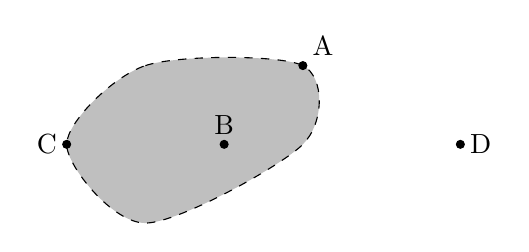
\begin{tikzpicture}
          \draw[fill=lightgray, dashed] plot [smooth cycle] coordinates {(0,0) (1,1) (3,1) (3,0) (1,-1)};
          \draw [fill] (3, 1) circle [radius=0.05];
          \node [above right] at (3,1) {A};
          \draw [fill] (2,0) circle [radius=0.05];
          \node [above] at (2,0) {B};
          \draw [fill] (0,0) circle [radius=0.05];
          \node [left] at (0,0) {C};
          \draw [fill] (5,0) circle [radius=0.05];
          \node [right] at (5, 0) {D};
        \end{tikzpicture}
        \caption{Points $A, B, C$ are limit points of the open set. }
        \label{fig:limit_boundary}
      \end{figure}

      \item A point can be at the ``convergence point'' of a sequence. 
      \begin{figure}[H]
        \centering 
        \begin{tikzpicture}
          \draw [fill] (0, 2.2) circle [radius=0.05];
          \draw [fill] (1, 2.4) circle [radius=0.05];
          \draw [fill] (2, 2) circle [radius=0.05];
          \draw [fill] (2.5, 1.8) circle [radius=0.05];
          \draw [fill] (2.6, 1.6) circle [radius=0.05];
          \draw [fill] (2.65, 1.67) circle [radius=0.05];
          \draw [fill] (2.654, 1.64) circle [radius=0.05];
          \draw [fill] (2.6543, 1.63) circle [radius=0.05];
          \node [right] at (2.6543, 1.63) {p};
        \end{tikzpicture}
        \caption{Note that if $S$ is a sequence of points in $\mathbb{R}^{2}$ that converges to $p$ without ever hitting it, we can say that $p \not\in S$ is a limit point of $S$.}
        \label{fig:limit_sequence}
      \end{figure}
    \end{enumerate}
  \end{example}

  \begin{example}[Examples of Non-Limit Points]
    There are generally two instances of non-limit points. Let $X = \mathbb{R}$ and $S = (0, 1) \cup \{2\}$. 
    \begin{enumerate}
      \item $5$ is clearly not a limit point. 
      \item $2$, although in $S$, is not a limit point since we are talking about the punctured neighborhood. A point in $S$ that is not a limit point is called an \textbf{isolated point}. 
    \end{enumerate}
  \end{example}

  \begin{example}[Counterintuitive Limit Points in Lower Limit Topology]
    Note that given an interval $(a, b) \subset \mathbb{R}$ in the lower limit topology, $a$ is a limit point but $b$ is \textit{not} a limit point!
  \end{example}

  \begin{theorem}[Union of Limit Points is Limit Points of Union]
    Let $A_1, \ldots, A_n$ be a finite collection of sets. Then 
    \begin{equation}
      \bigcup_{i=1}^n A_i^\prime = \bigg( \bigcup_{i=1}^n A_i \bigg)^\prime
    \end{equation}
  \end{theorem}
  \begin{proof}
    Let the LHS be $W$ and the RHS be $V$. If $x \in W$, $x \in A_i^\prime$ for some $i$, and so for all $\epsilon > 0$, there exists a $B_\epsilon^\circ (x)$ s.t. 
    \begin{equation}
      B_\epsilon^\circ (x) \cap A_i \neq \emptyset \implies B_\epsilon^\circ (x) \cap \bigg( \bigcup_{i=1}^n A_i \bigg) \neq \emptyset
    \end{equation}
    which means that $x \in V$. Now assume that $x \in V$. Then for all $\epsilon > 0$, there exists a $B_\epsilon^\circ (x)$ s.t. 
    \begin{equation}
      B_\epsilon^\circ (x) \cap \bigg( \bigcup_{i=1}^n A_i \bigg) \neq \emptyset
    \end{equation}
    which implies that $B_\epsilon^\circ (x) \cap A_i \neq \emptyset$ for some $i$, which means that $x \in A_i^\prime \subset W$. 
  \end{proof}

  Note that this is clearly not true for infinite unions. Look at the countable set $\mathbb{Q} \subset \mathbb{R}$. Each $\{q\}^\prime = \emptyset$, but $\mathbb{Q}^\prime = \mathbb{R}$. Look at the uncountable set $\mathbb{R}$. Each $\{x \in \mathbb{R}\}^\prime = \emptyset$, but $\mathbb{R}^\prime = \mathbb{R}$. 

  \begin{definition}[Closed Set]
    A set $S \subset X$ is \textbf{closed}\footnote{Note that open and closed sets are not mutually exclusive. A set might be open, closed, both, or neither. A set that is both open and closed is called \textbf{clopen}.} if it satisfies either of the equivalent properties. 
    \begin{enumerate}
      \item Its complement $X \setminus S$ is open in $\T$. 
      \item It contains all of its limit points. 
    \end{enumerate}
  \end{definition}
  \begin{proof}
    We prove bidirectionally. 
    \begin{enumerate}
      \item ($\rightarrow$) Given that $S$ contains all its limit points, then let $x \in S^c$. $x$ is not a limit point of $S$ since if it were, then it would be in $S$, and so there exists a punctured open neighborhood $B_\epsilon^\circ (x)$ of $x$ s.t. $S \cap B_\epsilon^\circ (x) = \emptyset$. Since $x \not\in S$, we also have $S \cap B_\epsilon (x) = \emptyset$, which implies that $B_\epsilon (x) \subset S^c$. Since for every $x \in S^c$, there exists a $B_\epsilon (x) \subset S^c$, $S^c$ is open. 

      \item ($\leftarrow$) For simplicity, it suffices to prove if $S$ open, then $S^c$ is closed. Given that $S$ is open, we have for every $x \in S$, there exists $B_\epsilon (x) \subset S$, which implies that $B_\epsilon (x) \cap S^c = \emptyset$. Since there exists an $B_\epsilon (x)$ that does not contain points in $S^c$, $x$ cannot be a limit point of $S^c$, and so there exists no limit points of $S^c$ in $S$. Therefore, all limit points of $S^c$ are in $S^c$, proving that $S^c$ is closed.  
    \end{enumerate}
  \end{proof}
  
  \begin{theorem}[Topological Space wrt Closed Sets]
    Let $X$ be a topological space. Then, the following conditions hold
    \begin{enumerate}
      \item $\emptyset$ and $X$ are clopen.
      \item Arbitrary intersections of closed sets are closed. 
      \item Finite unions of closed sets are closed. 
    \end{enumerate}
  \end{theorem}
  \begin{proof}
    Listed. 
    \begin{enumerate}
      \item Let $x$ be a limit point of $\cap_\alpha F_\alpha$, and we want to show that $x \in \cap_\alpha F_\alpha$. By definition of limit points, for every $\epsilon > 0$, we have 
      \begin{equation}
        B_\epsilon (x) \cap \bigg( \bigcap_\alpha F_\alpha \bigg)
      \end{equation}
      which means that $B_\epsilon (x) \cap F_\alpha \neq \emptyset$ for all $\alpha$. This means that $x$ is a limit point for every $F_\alpha$, and since they are all closed, $x \in F_\alpha$ for all $\alpha$, which implies that $x \in \cap_\alpha F_\alpha$. 
    \end{enumerate}
  \end{proof}

\subsection{Dense Subsets}

  \begin{definition}[Dense Subsets]
    Let $S \subset (X, \mathscr{T})$. $S$ is \textbf{dense} in $X$ if every point $p \in X$ is a limit point of $S$. In other words, for any point $p \in X$ and any open neighborhood $U_p$ of $p$, $U_p \cap S$ is nontrivial. Otherwise, $p$ is a point of $S$. 
  \end{definition}

  The following example is a crucial fact for proving further properties of topological spaces. 

  \begin{example}
    $\mathbb{Q}^{n}$ is a dense set of $\mathbb{R}^{n}$ with the open ball topology. If we have the discrete topology of $\mathbb{R}^{2}$, an open neighborhood of a point is the point itself, so no limit points would exist beyond the points in $S$ itself. So $\mathbb{Q}^{n}$ is not dense in $\mathbb{R}^{n}$ with this topology. 
  \end{example}

\subsection{Interiors and Closures}

  Now that we've determined limit points, we would like to extend sets into their limit points. The process of doing this is called the \textit{closure} of a set. 

  \begin{definition}[Closure]
    The \textbf{closure} of set $S$ is $\overline{S}$ is defined in the following equivalent ways. 
    \begin{enumerate}
      \item $\overline{S} = S \cup S^\prime$, i.e. the union of itself and its limit points. 
      \item $\overline{S}$ is the intersection of all closed sets $C$ containing $S$. 
    \end{enumerate}
  \end{definition}
  \begin{proof}
    
  \end{proof}

  \begin{theorem}
    If $X$ is a metric space and $E \subset X$, then 
    \begin{enumerate}
      \item $\overline{E}$ is closed. 
      \item $E = \overline{E}$ if and only if $E$ is closed. 
      \item $\overline{E} \subset F$ for every closed set $F \subset X$ such that $E \subset F$. That is, if $E \subset F$ closed, then ``increasing" the size of $E$ to its closure will not make it greater than $F$. 
    \end{enumerate}
  \end{theorem}
  \begin{proof}
    Listed. 
    \begin{enumerate}
      \item Let $x$ be a limit point of $\overline{E}$. Then, for every $\epsilon > 0$, we have $B_\epsilon (x) \cap \overline{E} \neq \emptyset$, which means that either $B_\epsilon (x) \cap E \neq \emptyset$ (in which case $x \in E^\prime \implies x \in \overline{E}$ and we are done) or $B_\epsilon (x) \cap E^\prime \neq \emptyset$. We wish to prove that in the latter case, $x$ being a limit point of $E^\prime$ still implies that $x$ is a limit point of $E$. Since $B_\epsilon (x) \cap E^\prime \neq \emptyset$, there must exist a $y \in B_\epsilon (x) \cap E^\prime$. Since $y \in E^\prime$, we can construct an open ball $B_\delta (y)$ containing elements of $E$, and since $B_\epsilon (x)$ is open, we can contain $B_\delta (y)$ entirely within $B_\epsilon (x)$. Therefore, 
      \[B_\delta (y) \cap E \neq \emptyset \implies B_\epsilon (x) \cap E \neq \emptyset\]
      therefore, $x \in E^\prime \implies x \in \overline{E}$. 

      \item If $E$ is closed, then $E^\prime \subset E \implies \overline{E} = E \cup E^\prime = E$. If $E = \overline{E} = E \cup E^\prime$, then $E^\prime \subset E \implies E$ is closed. 

      \item Since $E \subset F$, it suffices to prove that $E^\prime \subset F$. Consider a limit point $x$ of $E$. Then every punctured open neighborhood of $x$ satisfies $B_\epsilon^\circ (x) \cap E \neq \emptyset$. But since $E \subset F$, we have 
      \[B_\epsilon^\circ (x) \cap F \neq \emptyset\]
      and so $x$ is also a limit point of $F$. But since $F$ is closed, $x \in F$. Therefore, $\overline{E} = E \cup E^\prime \subset F$. 
    \end{enumerate}
  \end{proof}

  The first two statements (1) and (2) imply the following. 

  \begin{corollary}
    The closure of the closure of $E$ is equal to the closure of $E$. 
  \end{corollary}
  \begin{proof}
    We know that $\overline{\overline{E}} \supset \overline{E}$, so we must prove that $\overline{\overline{E}} \subset \overline{E}$, which is equivalent to proving that $\overline{E}^\prime \subset \overline{E}$. Let $x \in \overline{E}^\prime$, i.e. is a limit point of $\overline{E}$. Then, for every $\epsilon > 0$, we have $B_\epsilon (x) \cap \overline{E} \neq \emptyset$. Pick a point $y$ from this intersection, and since $B_\epsilon (x)$ is open, we can construct an open ball $B_\delta (y)$ fully contained in $B_\epsilon (x)$. Since $y \in \overline{E}$, $y$ is a limit point of $E$, which implies 
    \begin{equation}
      B_\delta (y) \cap E \neq \emptyset \implies B_\epsilon (x) \cap E \neq \emptyset
    \end{equation}
    and therefore $x$ is a limit point of $E$, $x \in \overline{E}$. 
  \end{proof}
  

  \begin{example}
    If $S$ is an open ball, $\Bar{S}$ is the closed ball. 
  \end{example}

  From semantics, it may seem like the interior and exterior (defined later) are related, but from a mathematical point of view, the interior and closure are dual notions. 

  \begin{definition}[Interior]
    Let $S \subset X$. Then, the following definitions of the \textbf{interior} of $S$, denoted $S^\circ$, are equivalent. 
    \begin{enumerate}
      \item $x \in S^\circ$ if $\exists U_x \ni x$ s.t. $U_x \subset S$. 
      \item $S^\circ$ is the union of all open sets contained in $S$. 
      \item $S^{o}$ is the complement of the closure of the complement of S. 
      \begin{equation}
        S^{o} = \big(\overline{S^{c}}\big)^{c}
      \end{equation}
    \end{enumerate}
  \end{definition}
  \begin{proof}
    
  \end{proof}

  An interior point means that we can always contain the point in $S$ with some ``breathing room." By definition an open set is a set where all of its points are interior points. A set is then said to be open if every point has this breathing room. This can be useful when defining differentiation at a point within an open set, since we can always find a neighborhood to take limits on. 

  \begin{lemma}[Open and Closed in Terms of Interiors and Closures]
    Let $S$ be a subset of some topological space $X$. 
    \begin{enumerate}
      \item $S$ is open iff $S = S^{o}$. $S^{o}$ is always open.
      \item $S$ is closed iff $S = \overline{S}$. $\overline{S}$ is always closed. 
    \end{enumerate}
  \end{lemma}

  \begin{theorem}[Clopen sets in Reals]
    There are no proper clopen sets in $\mathbb{R}$. 
  \end{theorem}

\subsection{Exteriors and Boundaries}

  \begin{definition}[Exteriors]
    Let $S \subset X$. The \textbf{exterior} of $S$, denoted $S^e$, is defined in the following equivalent ways.\footnote{We can informally think of the exterior being strictly outside of $S$ and its boundary.}
    \begin{enumerate}
      \item $S^e$ is the complement of the closure of $S$. 
      \item $S^e$ is the interior of the complement of $S$. 
    \end{enumerate}
  \end{definition}
  \begin{proof}
    
  \end{proof}

  \begin{definition}[Boundary]
    Let $S \subset X$. The \textbf{boundary} of $S$, denoted $\partial S$, is defined in the following equivalent ways. 
    \begin{enumerate}
      \item $\partial S$ is the closure minus the interior of $S$ in $X$. 
      \item $\partial S$ is the intersection of the closure of $S$ with the closure of its complement, i.e the set of all points $x$ such that every neighborhood $U_x$ intersects both the interior and exterior. 
      \item $\partial S$ is the set of points that are neither in the exterior nor the interior. 
      \item $x \in \partial S$ if every neighborhood of $x$ intersects both the interior and exterior of $S$. 
    \end{enumerate}
  \end{definition}
  \begin{proof}
    
  \end{proof}

  From the above, we get the intuitive notion that these three parts divide up the whole space. 

  \begin{theorem}[Partitioning of Space]
    Given $S \subset X$, $X$ is partitioned into the interior, boundary, and exterior of $S$. 
    \begin{equation}
      X = S^\circ \sqcup \partial S \sqcup S^e
    \end{equation}
  \end{theorem}
  \begin{proof}
    The fact that 
  \end{proof}

  One counterintuitive result is the \href{https://en.wikipedia.org/wiki/Lakes_of_Wada}{Lakes of Wada}, which are three disjoint connected open sets of the open unit square $(0, 1)^2$ with the property that they \textit{all} have the same boundary. In other words, for any point selected on the boundary of one of the lakes, the other two lakes' boundaries also contain that point. 

\subsection{Basis} 

  We want to continue analyzing the properties of a topology, but sometimes working with the entire topology is a bit thorny. There is a tamer representation of a topology, which can also give us the starting point to \textit{construct} topologies. 

  \begin{definition}[Basis] 
    \label{def:basis}
    If $X$ is a set, a \textbf{basis} on $X$ is a collection $\B$ of subsets of $X$ (called \textbf{basis elements}) such that
    \begin{enumerate}
      \item For each $x \in X$, there is at least one basis element $B \in \B$ containing $x$. That is, the elements of $\B$ covers $X$. 
      \item If $x$ belongs to the intersection of two basis elements $B_1$ and $B_2$, then there is a basis element $B_3$ containing $x$ such that $B_3 \subset (B_1 \cap B_2)$. 
    \end{enumerate}
  \end{definition} 

  The name gives away the clue that a topology may be created from this basis.  

  \begin{definition}[Basis to Topology]
    \label{def:basis-to-topology}
    Given a basis $\B$ on a set $X$, we can define a topology $\T$, called the \textbf{topology generated by $\B$}, in the following equivalent ways. 
    \begin{enumerate}
      \item $\T$ consists of subsets $U$ of $X$ satisfying the property that for each $x \in U$, there exists a basis element $B \in \B$ such that $x \in B \subset U$.\footnote{Note that since we can always set $U = \emptyset$, the basis doesn't need to contain $\emptyset$. }
      \begin{center}
        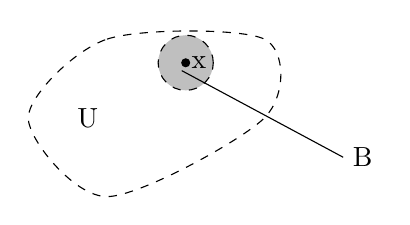
\begin{tikzpicture}
        \draw[dashed] plot [smooth cycle] coordinates {(0,0) (1,1) (3,1) (3,0) (1,-1)};
        \node [right] at (0.5,0) {U};
        \draw[fill=lightgray,dashed] (2,0.7) circle [radius=0.35];
        \draw[fill] (2, 0.7) circle [radius=0.05];
        \node [right] at (1.95,0.7) {x};
        \node [right] at (4,-0.5) {B};
        \draw (1.95,0.6)--(4,-0.5);
        \end{tikzpicture}
      \end{center}

      \item $\T$ consists of all possible unions of elements in $\B$. 
      \begin{equation}
        \T \coloneqq \Big\{ \bigcup_i B_i \mid B_i \in \B\Big\}
      \end{equation}
    \end{enumerate}
  \end{definition} 
  \begin{proof}
    We prove that the 2 methods generate a topology, and then finally prove that it they are the same topology. 
    \begin{enumerate}
      \item Clearly, $\emptyset$ and $X$ itself are in $\T$. To prove property 2, given a certain indexed family of subsets $\{U_\alpha\}_{\alpha \in I}$ of $\T$, we must show that 
      \begin{equation}
        U = \bigcup_{\alpha \in I} U_\alpha \in \T
      \end{equation}
      Given $x \in U$, there exists at least one index $\alpha$ such that $x \in U_\alpha$. Since $U_\alpha \in \T$ already, there exists a basis element $b \in \B$ such that $x \in b \subset U_\alpha$. But 
      \begin{equation}
        U_\alpha \subseteq U \implies b \subset U
      \end{equation}
      So, by definition, any arbitrary union of $U$ of these subsets is also in $\T$. 

      To prove property 3, we must show that 
      \begin{equation}
        W = \bigcap_{\alpha \in I} U_\alpha \in \T
      \end{equation}
      Given $x \in W$, by definition of a basis element, there exists a $b \in \B$ such that 
      \begin{equation}
        x \in b \subset (U_\beta \cap U_\gamma) \forall \beta, \gamma \in I \implies \text{ there exists } \Tilde{b} \in \B \text{ s.t. } x \in \Tilde{b} \subset \bigcap_{\alpha \in I} U_\alpha
      \end{equation}
      By definition, $W$ is also open. Since this arbitrary set of subsets $\T$ suffices the 3 properties, it is a topology of $X$ by definition. 

      \item $(\rightarrow)$ Given a collection of elements in $\B$, they are also elements of $\T$. Since $\T$ is a topology, their union in also in $\T$. 

      $(\leftarrow)$ Given an open set $U \in \T$, for every point $x \in U$, by definition we can choose a basis element $b \in \B$ such that $x \in b \subset U$. Then, the union of all these basis elements is by definition $b$. 
        
    \end{enumerate}
  \end{proof}

  We have learned how to go from a basis to a topology. The following lemma tells us how to identify a basis within a topology. 

  \begin{theorem}[Topology to Basis]
    Let $(X, \T)$ be a topological space, and let $\B$ be a collection of open subsets of $X$ such that for every open set $U$ and each $x \in U$, there exists an element $B \in \B$ such that
    \begin{equation}
      x \in B \subset U
    \end{equation}
    Then, $\B$ is a basis for the topology of $X$. 
  \end{theorem}
  \begin{proof}
    Note that there are two claims here: $\B$ is a basis and the topology that $\B$ generates is equal to $\T$. 
    \begin{enumerate}
      \item To prove that $\B$ is a basis, note that $X$ is an open set, and by assumption, for every $x \in X$, there exists a $B \in \B$ s.t. $x \in B \subset X$. Therefore $\B$ covers $X$. Now take two basis elements $B_1, B_2 \in \B$ with $x \in B_1 \cap B_2$. Since we know that $B_1, B_2$ are open, $B_1 \cap B_2$ is open and so for each $x \in B_1 \cap B_2$, there exists a basis element $B_3$ s.t. $x \in B_3 \in (B_1 \cap B_2)$. Thus $\B$ is a basis. 

      \item Let us call $\T^\prime$ the topology generated by $\B$. Then, given $U \in \T$, by assumption for any $x \in U$, there exists a basis element $B \in \B$ s.t. $x \in B \subset U$, so $x \in \T^\prime$. Conversely, if $U \in \T^\prime$, then $U$ is an arbitrary union of elements $B \in \B$ where each $B$ is open in $\T$, so $U \in \T$. So $\T = \T^\prime$. 
    \end{enumerate}
  \end{proof} 

  Characterizing topologies in terms of basis is quite effective since we can work with more manageable sets. 

  \begin{lemma}[Fineness w.r.t. Basis]
    Given two topologies $\T$ and $\T^\prime$ with their bases $\B$ and $\B^\prime$, respectively, the following are equivalent. 
    \begin{enumerate}
      \item $\T^\prime$ is finer than $\T$. 
      \item For each $x \in X$ and basis element $B \in \B$ containing $x$, there exists a basis element $B^\prime \in \B^\prime$ such that $x \in B^\prime \subset B$. 
    \end{enumerate}
  \end{lemma}

  So we have seen how we can take a collection of sets satisfying the basis properties and construct a topology as the union of the sets in this collection. What happens if we can relax some of these conditions? Note that the first condition was that the basis elements must cover $X$. This is non-negotiable. However, if we remove the second requirement that a basis element must be contained in an intersection of basis elements, we can get a \textit{subbasis}. 

  \begin{definition}[Subbasis]
    A \textbf{subbasis} $\mathscr{S}$ for a topology on $X$ is a collection of subsets of $X$ whose union is equal to $X$. 
  \end{definition}

  \begin{theorem}[Subbasis to Topology]
    Given a subbasis $\mathscr{S}$ on a set $X$, the \textbf{topology generated by $\mathscr{S}$} is defined to be the collection $\T$ of all unions of finite intersections of elements of $\mathscr{S}$. 
  \end{theorem}
  \begin{proof}
    It suffices to show that the collection of finite intersections of elements form a basis. 
  \end{proof}

  Now we show three extremely common topologies that can be constructed with bases. 

\subsubsection{Order Topology}

  \begin{definition}[Order Topology]
    \label{def:order-topology}
    Let $X$ be a set with a simple order relation. Let $\B$ be the collection of all sets of the following types.\footnote{If $X$ has no minimum or maximum, then there are no sets of type of 2 or 3, respectively.}
    \begin{enumerate}
      \item All open intervals $(a, b) \coloneqq \{x \in X \mid a < x < b\} \subset X$
      \item All half-open intervals $[a_0, b)$, where $a_0$ is the minimum element of $X$
      \item All half-open intervals $(a, b_0]$, where $b_0$ is the maximum element of $X$. 
    \end{enumerate}
    This set $\B$ is a basis for the \textbf{order topology} of $X$. 
  \end{definition}
  \begin{proof}
    We prove that this set $\mathscr{B}$ is a basis. 
    \begin{enumerate}
      \item It covers $X$. If $x \in X$ is the maximum or minimum we can cover it with $(a, b_0]$ and $[a_0, b)$, respectively. If not, then $x$ is bounded above and below, and so there exists $a, b \in X$ s.t. $a < x < b \implies x \in (a, b)$. 

      \item Let $x \in (a_1, b_1)$ and $x \in (a_2, b_2)$. Then, 
      \begin{equation}
        x \in (\max\{a_1, a_2\}, \min\{b_1, b_2\}) \in \mathscr{B} 
      \end{equation}
    \end{enumerate}
    Therefore, the generated collection is indeed a topology. 
  \end{proof}

  \begin{example}[Standard Order Topology on $\mathbb{R}$]
    The standard topology on $\mathbb{R}$ is precisely the order topology derived from the usual order on $\mathbb{R}$. Since $\mathbb{R}$ has no minimum or maximum, the basis consists of open intervals $(a, b) \subset \mathbb{R}$ with $a, b \in \mathbb{R}$. 
  \end{example}

  \begin{example}[Basis of Open Intervals with Rational Endpoints]
    We can however get away with smaller basis that generate the same topology on $\mathbb{R}$. If we take the set of all open intervals $(a, b) \subset \mathbb{R}$ with $a, b \in \mathbb{Q}$, this is also a basis for the same standard order topology. Too see why, let us denote this basis as $\B^\prime$ and the basis of all open intervals with real endpoints be $\B$. Then, clearly $B^\prime \subset \B \implies \T^\prime \subset \T$. As for the other, way, let us take an open interval $(a, b) \in \B$. Then we can see that 
    \begin{equation}
      (a, b) = \bigcup_{\substack{p, q \in \mathbb{Q} \\ a < p, q < b}} (p, q)
    \end{equation}
    where equality follows from density of rationals in $\mathbb{R}$. 
  \end{example}

  \begin{example}[$\mathbb{R}^2$ with Dictionary Order]
    Given $\mathbb{R} \times \mathbb{R}$ with the dictionary order, then $\mathbb{R} \times \mathbb{R}$ has neither a largest nor smallest element. Therefore, the order topology on $\mathbb{R} \times \mathbb{R}$ consists of all "intervals" of form
    \begin{equation}
      \big((a, b), (c, d) \big) \coloneqq  \{(x, y) \in \mathbb{R}^2 \mid (a, b) < (x, y) < (c, d)\}
    \end{equation}

    \begin{figure}[H]
      \centering 
      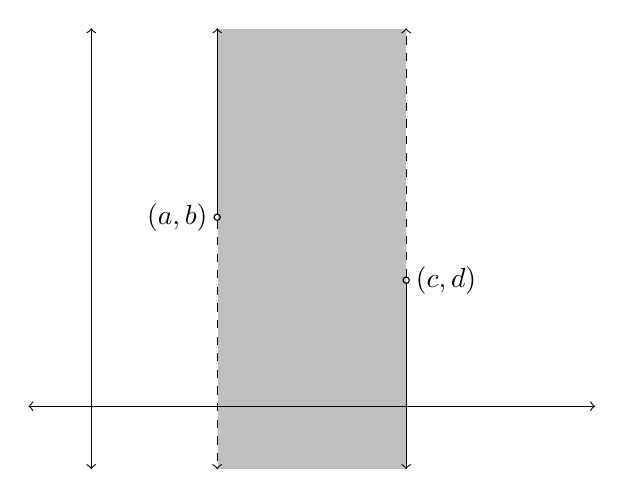
\begin{tikzpicture}[scale=0.8]
        \draw[white, fill=lightgray] (2,-1) rectangle (5,6);
        \draw[<->] (-1,0)--(8,0);
        \draw[<->] (0,-1)--(0,6);
        \draw[->] (2,3.05)--(2,6);
        \draw[->] (5,1.95)--(5,-1);
        \draw (2,3) circle [radius=0.05];
        \draw (5,2) circle [radius=0.05];
        \draw[dashed, ->] (2,2.95)--(2,-1);
        \draw[dashed,->] (5,2.05)--(5,6);
        \node[left] at (2,3) {$(a, b)$};
        \node[right] at (5,2) {$(c,d)$};
      \end{tikzpicture}
      \caption{This means that open rays and lines are also a part of the topology of $\mathbb{R} \times \mathbb{R}$. } 
      \label{fig:r2_dict_order}
    \end{figure}
  \end{example}

  \begin{example}[Positive Integers]
    The set of positive integers $\mathbb{Z}_+$ form an ordered set with a smallest element. The order topology for $\mathbb{Z}_+$ is precisely the discrete topology since every one-point set is an open set. 
    \begin{equation}
      \{n\} = (n-1, n+1)
    \end{equation}
  \end{example}

  \begin{example}[Two Copies of Positive Integers]
    The dictionary order topology on $\{1, 2\} \times \mathbb{Z}_+$ results in every one point set being open, except for the point $(2, 1)$. Since every neighborhood of $(2,1)$ must contain some point of form $(1, n)$ for arbitrarily large $n$, $\{(2,1)\}$ is not open. 
  \end{example}

  \begin{definition}
    If $X$ is an ordered set a $a \in X$, then there are 4 subsets of $X$ called rays determined by $a$. 
    \begin{enumerate}
      \item $(a, +\infty)$ 
      \item $(-\infty, a)$
      \item $[a, +\infty)$
      \item $(-\infty, a]$
    \end{enumerate}
    The first two sets are called \textbf{open rays}, and the latter two sets are called \textbf{closed rays}. 
  \end{definition}

  We can extend the basis of open intervals to some other basis based on the order, which generates other topologies. 

  \begin{example}[Lower/Upper Limit Topology]
    Given a totally ordered set $(X, \leq)$, 
    \begin{enumerate}
      \item the \textbf{lower limit topology} is the topology generated by the basis of all half-closed half-open intervals of form 
      \begin{equation}
        [a, b) \coloneqq \{ x \in X \mid a \leq x < b \}
      \end{equation}
      \item the \textbf{upper limit topology} is the topology generated by the basis of all half-open half-closed intervals of form 
      \begin{equation}
        (a, b] \coloneqq \{ x \in X \mid a < x \leq b \}
      \end{equation}
    \end{enumerate}
  \end{example}

  \begin{example}[Nested Interval Topology]
    In the space $X = (0,1)$, the \textbf{nested interval topology} is the topology generated by the basis of nested intervals of the form 
    \begin{equation}
      \B_{ni} \coloneqq \{ (0, 1-\frac{1}{n}) \mid n \in \mathbb{N} \}
    \end{equation}
  \end{example}

  A topology generated by closed intervals can also be a topology! 

  \begin{example}[Closed Interval Topology]
    In the set $X = [-1, 1]$, the following set 
    \begin{equation}
      \B_{ci} \coloneqq \{ [-1, a) \mid a > 0 \big\} \bigcup \big\{ (b, 1] \mid b<0 \}
    \end{equation}
    is a basis. The topology it generates is called the \textbf{closed interval topology}, denoted $\T_{ci}$. 
  \end{example}

  Finally, we talk about a seemingly arbitrary topology called the K-topology, but it is useful for counterexamples.   

  \begin{example}[K-Topology]
    In $\mathbb{R}$, let us denote $K = \{1/n\}_{n \in \mathbb{N}}$. Then the \textbf{K-topology} on $\mathbb{R}$ is the topology generated by the basis consisting of 
    \begin{enumerate}
      \item all open intervals $(a, b)$ with $a, b \in \mathbb{R}$. 
      \item all sets of the form $(a, b) \setminus K$ with $a, b \in \mathbb{R}$. 
    \end{enumerate}
  \end{example} 

  Now that we have some collection of topologies, let's try to compare them. We claim the following. 

  \begin{theorem}[Comparison of Topologies of the Real Line]
    
  \end{theorem}

\subsubsection{Metric Topology}

  For common sets like $\mathbb{R}^n$, which has an inner product, or $\mathbb{Q}$, which has an order, it is easy to build these topologies with set-builder notation. Consider the following. 

  \begin{definition}[Metric Topology]
    \label{def:metric-topology}
    Given a metric space $(X, d)$, let us denote the \textbf{metric topology}, or \textbf{open-ball topology}, as the set of subsets $U$ satisfying the property that for all $x \in U$, there exists a positive $r \in \mathbb{R}$ such that $B(x, r) \subset U$, where $B(x, r) \coloneqq \{y \in X \mid d(x, y) < r\}$ is the open ball of radius $r$ around $x$. We claim that this is a topology. 
  \end{definition} 
  \begin{proof}
    We show that the properties of a topology hold. 
    \begin{enumerate} 
      \item For the empty set, the inclusion of an open ball for a point in $\emptyset$ is vacuously satisfied. For the whole set, we choose any point $x$ and any $r$, and the open ball is trivially a subset of $X$. 

      \item Let $\{U_\alpha\}_{\alpha \in I}$ be a collection of open subsets of $X$. Let their union be denoted $U$. We claim $U$ is open. Pick any point $x \in U$. Then by definition of union, there exists some $\alpha \in I$ s.t. $x \in U_\alpha$. Since $U_\alpha$ is open, there exists a $r > 0$ s.t. $B(x, r) \subset U_\alpha \subset U$. Therefore $U$ is open. 

      \item Let $U_1, \ldots, U_k$ be open, and let us denote their intersection as $U$. We claim $U$ is open. Pick a point $x \in U$. Then for each $i = 1, \ldots, k$, $x \in U_i$ and there exists a corresponding $r_i > 0$  such that the open ball $B(x, r_i) \subset U_i$. Take the set $R = \{r_i\}$, which is a finite set living in $\mathbb{R}$. We will take for granted that every finite subset of an ordered set has a minimum.\footnote{If we wish to prove it, we can start with a singleton set, claim that its minimum is the only element. Then we use induction by assuming for a set $R$ of size $k$ that a minimum exists, and by adding $1$ more element $r$ we update the minimum to be $\min\{r, \min{R}\}$ and show that this is indeed the minimum.} Let us denote $r^\ast = \min{R}$, and we claim that $r^\ast$ gives us a ball that can fit inside $U$. Assume $y \in B(x, r^\ast)$. Then 
      \begin{align}
        y \in B(x, r^\ast) & \implies d(x, y) < r^\ast \\ 
                           & \implies d(x, y) < \min{R} \\
                           & \implies d(x, y) < r_i \text{ for } i = 1, \ldots, k \\
                           & \implies y \in B(x, r_i) \text{ for } i = 1, \ldots, k
      \end{align} 
      Since $B(x, r_i)$ by construction is contained within $U_i$, $y \in U_i$ for all $i$. This means by definition of intersection that $y \in U$, and we have proven that $B(x, r^\ast)$ completely fits inside $U$. 
    \end{enumerate}
  \end{proof} 

  Note that while open balls are used to define whether a set is open or not, the definition doesn't state whether open balls themselves are open sets. It turns out that it is easy to prove that they are. 
  
  \begin{lemma}[Open Balls are Open Sets]
    The open ball wrt any metric $d$ is an open set wrt the metric topology. 
  \end{lemma}
  \begin{proof}
    Let $y \in B(x, r)$. Then $d(x, y) < r \implies 0 < r - d(x, y)$. To show that $B(x, r)$ is open, we would like to show that there exists some $r^\prime > 0$ s.t. $y \in B(y, r^\prime) \subset B(x, r)$. Set $r^\prime = r - d(x, y)$. Then 
    \begin{align}
      z \in B(y, r^\prime) & \implies d(y, z) < r - d(x, y) \\
                           & \implies d(x, y) + d(x, y) < r \\
                           & \implies d(x, z) < r \\
                           & \implies z \in B(x, r)
    \end{align} 
    and so $B(y, r^\prime) \subset B(x, r)$. We are done. 
  \end{proof}

  \begin{example}[Discrete Metric Induces Discrete Topology]
    Given a set $X$, induce the metric $d$ defined
    \begin{equation}
      d(x, y) \coloneqq \begin{cases} 1 & \text{if } x \neq y \\ 0 & \text{if } x = y \end{cases}
    \end{equation}
    This metric induces the discrete topology on $X$, since the basis elements of the open balls
    \begin{equation}
      B_r (x) \coloneqq \{ y \in X \mid d(x, y) <r\}
    \end{equation}
    consists of two types of open sets. When $r \leq 1$, then $B_r (x) = x$ (since the radius is $0$). If $r > 1$, then the open set is the entire space $X$. 
  \end{example} 

  While the behavior for finite sets are predictable under the metric topology, as soon we we get into infinite sets, the properties of the metric topology may differ. 

  \begin{example}[Metric Topologies on $\mathbb{Z}$ and $\mathbb{Q}$]
    $\mathbb{Z}$ and $\mathbb{Q}$ are countable sets, so there is a bijection between them. If we give each of them the metric topology, $\mathbb{Z}$ ends up having the discrete topology (take the $0.5$-ball around each integer), whereas for $\mathbb{Q}$, we will see later that by the density of the rationals there are an infinite number of rationals in $(q - r, q + r)$ for $q \in \mathbb{Q}$. Therefore, the metric topology may or may not induce the discrete topology. 
  \end{example}

  \begin{example}[Supremum Norm in $\mathbb{R}^3$]
    \begin{figure}[H]
      \centering 
      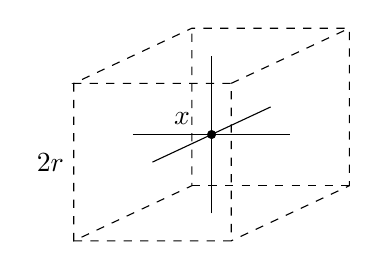
\begin{tikzpicture}
        \draw[dashed] (0,0)--(2,0)--(2,2)--(0,2)--(1.5,2.7)--(3.5,2.7)--(3.5,0.7)--(2,0);
        \draw[dashed] (2,2)--(3.5,2.7);
        \draw[dashed] (0,2)--(0,0)--(1.5,0.7)--(1.5,2.7);
        \draw[dashed] (1.5,0.7)--(3.5,0.7);
        \draw (1,1)--(2.5,1.7);
        \draw (0.75,1.35)--(2.75,1.35);
        \draw (1.75,0.35)--(1.75,2.35);
        \draw[fill] (1.75,1.35) circle (0.05);
        \node[above left] at (1.6,1.35) {$x$};
        \node[left] at (0,1) {$2r$};
      \end{tikzpicture}
      \caption{In $\mathbb{R}^3$, each basis element is a cube centered at $x$ with side lengths $2r$.} 
      \label{fig:sup_norm_R3}
    \end{figure}
  \end{example}

  \begin{theorem}[Metric Topologies on Finite Sets]
    If $(X, d)$ is a finite metric space, then the metric topology on it is the discrete topology. 
  \end{theorem}
  \begin{proof}
    Take all pairwise points and compute $\epsilon = \min_{x \neq y} \{d(x, y)\}$. Since $X$ is finite, all pairs are finite and therefore the minimum exists. Now let us take the $\epsilon$-ball around $x$. Then every $y \neq x$ has distance $d(x, y) \geq \epsilon$, and therefore $y \not\in B(x, \epsilon)$. So all single points are open sets, which induces the discrete topology. 
  \end{proof}

  A finite set $S$ of points does not have any limit points, since if we draw small enough circles around a $p \in S$, then at some point the circle will not contain any more points (remember that we're talking about deleted neighborhoods). Following this, we can deduce that a limit point must always have an infinite number of points close to it, as in no matter how small the circle gets, there are always an infinite number of points contained within that circle. This also means that if $p$ is a limit point, then we can construct a sequence of points in $S$ that converges to $p$, since every open ball with smaller and smaller radii will still have points in $S$.

  \begin{theorem}[Neighborhood of Limit Point Contains Infinite Points in Metric Space]
    Let $X$ be a metric space. If $p$ is a limit point of $S$, then every neighborhood of $p$ contains infinitely many points of $S$. The converse is also true trivially. 
  \end{theorem}
  \begin{proof}
    Assume $p$ is a limit point and that there exists a finite number of points within a deleted neighborhood $B_r^\circ (p)$. Then, we can enumerate them $p_1, p_2, \ldots, p_n$ by their distances to $p$, with 
    \begin{equation}
      d(p_1, p) \leq d(p_2, p) \leq \ldots \leq d(p_n, p)
    \end{equation}
    Since $p_1 \neq p$, we have $d(p_1, p) > 0$ and so, we can choose an $0 < \epsilon < d(p_1, p)$ s.t. $B_\epsilon^\circ (p)$ does not contain any of the $p_i$'s. This neighborhood does not contain any elements of $S$ and so $p$ is not a limit point. 
  \end{proof}

  \begin{corollary}[Finite Set in Metric Space has No Limit Points]
    Let $X$ be a metric space and $S = \{s_i\}_{i=1}^n$ be a finite set. Then, $S^\prime = \emptyset$.  
  \end{corollary}
  \begin{proof}
    If $S$ is a finite set, then every neighborhood of every point $p$ in $\mathbb{R}^n$ will have at most finite points, which, by the previous theorem, is not a limit point. 
  \end{proof}

  \begin{lemma}[Fineness of Metric Topologies]
    Let $d$ and $d^\prime$ be two metrics on the set $X$ with their respective induced topologies $\T, \T^\prime$. We claim that $\T \subset \T^\prime$ iff there exists a $M > 0$ s.t. 
    \begin{equation}
      d^\prime (x, y) < M \cdot d(x, y)
    \end{equation} 
    for all $x, y \in X$. That is, we can bound $d^\prime$ with a constant multiple of $d$. 
  \end{lemma}
  \begin{proof}
    
  \end{proof}

  More specifically, the metric topology generated by the $L_2$-metric on $\mathbb{R}^n$ is called the \textbf{Euclidean topology}. Note that the topological property of stability under countable intersection was required to show that the minimum of $R$ existed. This is not true for infinite sets in general. This gives us some motivation as to why we need the \textit{finite} intersection rather than an infinite one. 
  
  \begin{lemma}[Singletons are Not Open in $\mathbb{R}^n$]
    A singleton set is not open in $\mathbb{R}^n$ with the Euclidean topology.   
  \end{lemma}
  \begin{proof}
    We claim that the singleton set $S = \{0\}$ is not open under the Euclidean metric. We pick a point in $S$, which can only be $0$. Assume that there exists an $r > 0$ s.t. $B(x, r) \subset S$. $\mathbb{R}$ is Archimedean, so there exists a natural number $N$ s.t. $0 < 1/N < r$. We construct the vector $v = (v_1, \ldots, v_n)$ s.t. $v_1 = 1/N$ and $v_i = 0$ everywhere else. The distance between $0$ and $v$ is 
    \begin{equation}
      \| v - 0 \| = \|v\| = \sqrt{(1/N)^2} = 1/N < r
    \end{equation} 
    so $v \in B(x, r)$. But $v \neq 0$, and by contradiction such an $r$ cannot exist. In $\mathbb{R}^n$ we consider the countable intersection of open balls (which we have proved in class are open sets) around $0$ of radius $1/N$ for $n \in \mathbb{N}$. We claim that 
    \begin{equation}
      \bigcap_{n \in \mathbb{N}} B(0, 1/n) = \{0\}
    \end{equation} 
    We see that $1/n$ must always be positive and so $\|0 - 0\| = 0 < 1/n$. Therefore the LHS $\supset $ RHS. To see that the intersection contains no other element, consider any vector $v \neq 0$. Then by definition of the metric, $d(v, 0) > 0$. By the Archimedean property, there exists a natural $N \in \mathbb{N}$ s.t. $0 < 1/N < d(v, 0)$, which means that $v \not\in B(0, 1/N)$, and so $v$ cannot be in the intersection. Therefore, the intersection must be $\{0\}$, and we have shown that $B_0$ is not open, so we are done. 
  \end{proof}

  \begin{theorem}[Metric Topology is Always Finer than Cofinite]
    For a metric space $(X, d)$, the metric topology is finer than the cofinite topology. 
  \end{theorem} 
  \begin{proof}
    Note that if $X$ is finite, then both are reduced to the discrete topologies. 
  \end{proof}

  While it is not surprising that a basis uniquely generates a topology, it is not immediately obvious \textit{what} the generated topology looks like. It turns out that many different bases may generate the same topology, and the concept of fineness allows us to compare these topologies more effectively. For example, if two topologies are both finer than the other, then they must be equal. 

  \begin{theorem}[Euclidean Topology on $\mathbb{R}^n$]
    \label{thm:lp-norms-euclidean-topology}
    $L^p$ norms all generate the same topology on $\mathbb{R}^n$. 
  \end{theorem}
  \begin{proof}
    We can show that 
    \begin{equation}
      n^q d_\infty \leq n^q d_2 \leq n^q d_1 \leq d_p \leq n^{-p} d_\infty
    \end{equation}
    where $q$ is the holder conjugate of $p$. Visually, we can see that every open ball in $(\mathbb{R}^n, d)$ (with the Euclidean metric) is the form to the left, while an open ball in $(\mathbb{R}^n, \rho)$ (with the square metric) is of form on the right. 
    \begin{center}
      \begin{tikzpicture}[scale=0.5]
        \draw [dashed] (1,0) circle [radius=2];
        \draw [dashed] (6,-2) rectangle (10,2);
        \draw [fill] (1,0) circle [radius=0.05];
        \node [above left] at (1,0) {x};
        \draw (1,0)--(3,0);
        \node [above] at (1.5,0) {r};
        \draw [fill] (8,0) circle [radius=0.05];
        \node [below right] at (8,0) {x};
        \draw (8,0)--(10,0);
        \draw (8,0)--(8,2);
        \node [right] at (8,1) {r};
        \node [above] at (9,0) {r};
      \end{tikzpicture}
    \end{center}
    Clearly, we can form any open set of any "shape" using any arbitrary combination of these "circles" or "squares," indicating that they generate the same topology. 
  \end{proof}

\subsection{Exercises}

  \begin{exercise}[Munkres 13.1]
    Let $X$ be a topological space; let $A$ be a subset of $X$. Suppose that for each $x \in A$ there is an open set $U$ containing $x$ such that $U \subset A$. Show that $A$ is open in $X$.
  \end{exercise}
  \begin{solution}[Munkres 13.1]
    Given a $x \in A$, let us label its open neighborhood as $U_x \subset A$. We claim that 
    \begin{equation}
      A = \bigcup_{x \in A} U_x
    \end{equation} 
    We prove bidirectionally. 
    \begin{enumerate}
      \item $A \subset \cup_{x \in A} U_x$. Let $y \in A$. Then there exists an open $U_y$ containing $y$. Since $U_y$ is in the union by construction. 
      \begin{equation}
        y \in U_y \subset \bigcup_{x \in A} U_x
      \end{equation}
      \item $\cup_{x \in A} U_x \subset A$. Let $y \in \cup_{x \in A} U_x$. Then there must be some $U_y$ in this union s.t. $y \in U_y$. But by construction $U_y \subset A$, so $y \in A$. 
    \end{enumerate}
    We are done. 
  \end{solution}

  \begin{exercise}[Munkres 13.2]
    Consider the nine topologies on the set $X = \{a, b, c\}$ indicated in Example 1 of \S12. Compare them; that is, for each pair of topologies, determine whether they are comparable, and if so, which is the finer.
  \end{exercise}
  \begin{solution}[Munkres 13.2] 
    Given the figure, we denote $\mathscr{T}_{i, j}$ as the topology in the $i$th row (from top) and $j$th column (from left) in the figure below. When I say for all $i, j$, I mean for all $i, j \in \{1, 2, 3\}$. 
    \begin{figure}[H]
      \centering 
      \includegraphics[scale=0.3]{img/top.png}
      \caption{} 
      \label{fig:top}
    \end{figure} 
    $\mathscr{T}_{11}$ is the indiscrete topology so $\mathscr{T}_{11} \subset \mathscr{T}_{i, j}$ for all $i, j$, i.e. it is coarsest. $\mathscr{T}_{33}$ is the discrete topology so $\mathscr{T}_{i, j} \subset \mathscr{T}_{3, 3}$ for all $i, j$, i.e. it is the finest. We list all other comparable topologies below. 
    \begin{enumerate}
      \item $\mathscr{T}_{1, 2} \subset \mathscr{T}_{3, 2}, \mathscr{T}_{1, 3}, \mathscr{T}_{2, 3}$. 
      \item $\mathscr{T}_{3, 1} \subset \mathscr{T}_{1, 2}, \mathscr{T}_{3, 2}, \mathscr{T}_{1, 3}, \mathscr{T}_{2, 3}$. 
      \item $\mathscr{T}_{1, 2} \subset \mathscr{T}_{3, 2}$. 
      \item $\mathscr{T}_{1, 3} \subset \mathscr{T}_{2, 3}$. 
    \end{enumerate}
  \end{solution}

  \begin{exercise}[Munkres 13.3]
    Show that the collection $\mathcal{T}_c$ given in Example 4 of \S12 is a topology on the set $X$. Is the collection
    \begin{align*}
      \mathcal{T}_\infty = \{U \mid X - U \text{ is infinite or empty or all of } X\}
    \end{align*}
    a topology on $X$?
  \end{exercise}
  \begin{solution}[Munkres 13.3]
    We denote $\mathcal{T}_c$ as the set of all subsets $U \subset X$ such that $X \setminus U$ is countable is all of $X$. We show the 4 properties: 
    \begin{enumerate}
      \item $U = \emptyset \implies X \setminus U = X$, which is by definition in $\mathcal{T}_c$. 
      \item $U = X \implies X \setminus U = \emptyset$, which has cardinality $0$. Therefore it is countable and is in $\mathcal{T}_c$. 

      \item Let $\{U_\alpha\}_{\alpha \in I} \in \mathcal{T}_c$ by a collection of open sets of $X$. Then 
      \begin{equation}
        X \setminus \bigcup_{\alpha \in I} U_{\alpha} = \bigcap_{\alpha \in I} (X \setminus U_\alpha)
      \end{equation}
      $X \setminus U_\alpha$ is countable for all $\alpha \in I$, so let us fix some $\alpha^\prime$. Then 
      \begin{equation}
        \bigcap_{\alpha \in I} (X \setminus U_\alpha) \subset U_{\alpha^\prime} \implies \bigg| \bigcap_{\alpha \in I} (X \setminus U_\alpha) \bigg| \leq \big| U_{\alpha^\prime} \big| 
      \end{equation}
      and so the intersection is also countable. 
      \item Let $\{U_i\}_{i=1}^n$ by a finite collection of open sets of $X$. Then 
      \begin{equation}
        X \setminus \bigcap_{i=1}^n U_i = \bigcup_{i=1}^n (X \setminus U_i)
      \end{equation}
      Since $U_i$ are open, $X \setminus U_i$ are countable, and since the finite union of countable sets are countable, the RHS is countable, which implies the LHS is countable and so $\cap_{i=1}^n U_i$ is open as well. 
    \end{enumerate}

    As for $\mathcal{T}_\infty$, it is not a topology. Let us take $X = \mathbb{R}$, and look at the sets $\mathbb{Z}_{\geq 0}, \mathbb{Z}_{\leq 0}$ consisting of all the non-negative and non-positive integers. They are both infinite, and so $\mathbb{R} \setminus \mathbb{Z}_{\geq 0}$ and $\mathbb{R} \setminus \mathbb{Z}_{\leq 0}$ are in $\mathcal{T}_\infty$. Consider their union. 
    \begin{equation}
      (\mathbb{R} \setminus \mathbb{Z}_{\geq 0}) \cup (\mathbb{R} \setminus \mathbb{Z}_{\leq 0}) = \mathbb{R} \setminus (\mathbb{Z}_{\geq 0} \cap \mathbb{Z}_{\leq 0}) = \mathbb{R} \setminus \{0\}
    \end{equation}
    But $\mathbb{R} \setminus (\mathbb{R} \setminus \{0\}) = \{0\}$, and so $\mathbb{R} \setminus \{0\}$ is not open. Therefore $\mathcal{T}_c$ doesn't satisfy the definition of a topology. 
  \end{solution}

  \begin{exercise}[Munkres 13.4]
    (a) If $\{\mathcal{T}_\alpha\}$ is a family of topologies on $X$, show that $\bigcap \mathcal{T}_\alpha$ is a topology on $X$. Is $\bigcup \mathcal{T}_\alpha$ a topology on $X$?
    
    (b) Let $\{\mathcal{T}_\alpha\}$ be a family of topologies on $X$. Show that there is a unique smallest topology on $X$ containing all the collections $\mathcal{T}_\alpha$, and a unique largest topology contained in all $\mathcal{T}_\alpha$.
    
    (c) If $X = \{a, b, c\}$, let
    \begin{align*}
      \mathcal{T}_1 = \{\emptyset, X, \{a\}, \{a, b\}\} \quad \text{and} \quad \mathcal{T}_2 = \{\emptyset, X, \{a\}, \{b, c\}\}.
    \end{align*}
    Find the smallest topology containing $\mathcal{T}_1$ and $\mathcal{T}_2$, and the largest topology contained in $\mathcal{T}_1$ and $\mathcal{T}_2$.
  \end{exercise}
  \begin{solution}
    
  \end{solution}

  \begin{exercise}[Munkres 13.5]
    Show that if $\mathcal{A}$ is a basis for a topology on $X$, then the topology generated by $\mathcal{A}$ equals the intersection of all topologies on $X$ that contain $\mathcal{A}$. Prove the same if $\mathcal{A}$ is a subbasis.
  \end{exercise}
  \begin{solution}
    
  \end{solution}

  \begin{exercise}[Munkres 17.1]
    Let $\mathcal{C}$ be a collection of subsets of the set $X$. Suppose that $\emptyset$ and $X$ are in $\mathcal{C}$, and that finite unions and arbitrary intersections of elements of $\mathcal{C}$ are in $\mathcal{C}$. Show that the collection
    \begin{align*}
      \mathcal{T} = \{X - C \mid C \in \mathcal{C}\}
    \end{align*}
    is a topology on $X$.
  \end{exercise}
  \begin{solution}
    
  \end{solution}

  \begin{exercise}[Munkres 17.2]
    Show that if $A$ is closed in $Y$ and $Y$ is closed in $X$, then $A$ is closed in $X$.
  \end{exercise}
  \begin{solution}
    
  \end{solution}

  \begin{exercise}[Munkres 17.3]
    Show that if $A$ is closed in $X$ and $B$ is closed in $Y$, then $A \times B$ is closed in $X \times Y$.
  \end{exercise}
  \begin{solution} 
    It suffices to prove that $(X \times Y) \setminus (A \times B)$ is open. 
    \begin{align}
      (X \times Y) \setminus (A \times B) & \coloneqq \{ (x, y) \in X \times Y \mid (x \not\in A) \lor (y \not\in B) \} \\
                                          & = \{(x, y) \in X \times Y \mid x \not\in A \} \cup \{(x, y) \in X \times Y \mid y \not\in B \} \\
                                          & = [(X \setminus A) \times Y] \cup [X \times (Y \setminus B)]
    \end{align}
    We know that since $A, B$ are closed, $X \setminus A, Y \setminus B$ are open. Therefore each the expressions under definition of the product topology are open and their union must also be open. 
  \end{solution}

  \begin{exercise}[Munkres 17.4]
    Show that if $U$ is open in $X$ and $A$ is closed in $X$, then $U - A$ is open in $X$, and $A - U$ is closed in $X$.
  \end{exercise}
  \begin{solution}
    We know that $U^c$ is closed and $A^c$ is open. Since $U \setminus A = U \cap A^c$, it is the finite intersection of two open sets and therefore is open. Since $A \setminus U = A \cap U^c$, is an intersection of two closed sets, it is closed. 
  \end{solution}

  \begin{exercise}[Munkres 17.5]
    Let $X$ be an ordered set in the order topology. Show that $\overline{(a, b)} \subset [a, b]$. Under what conditions does equality hold?
  \end{exercise}
  \begin{solution}
    
  \end{solution}

  \begin{exercise}[Munkres 17.6]
    Let $A$, $B$, and $A_\alpha$ denote subsets of a space $X$. Prove the following:
    \begin{enumerate}
      \item If $A \subset B$, then $\bar{A} \subset \bar{B}$.
      \item $\overline{A \cup B} = \bar{A} \cup \bar{B}$.
      \item $\bigcup \bar{A}_\alpha \supset \overline{\bigcup A_\alpha}$; give an example where equality fails.
    \end{enumerate}
  \end{exercise}
  \begin{solution}
    For the first part, let $x \in \overline{A}$. If $x \in A$, then $x \in B \subset \overline{B}$ and we are done. If $x \in A^\prime$, then by definition every punctured neighborhood $U_x^\circ$ has a nonempty intersection with $A$, i.e. $U_x^\circ \cap A \neq \emptyset$ for any $U_x$. Choose $y \in U_x^\circ \cap A$. Since $y \in A \subset B$, this means that $y \in U_x^\circ \cap B$, which proves that $A^\prime \subset B^\prime$. 

    For the second part, we show bidirectionally. 
    \begin{enumerate}
      \item $\overline{A} \cup \overline{B} \subset \overline{A \cup B}$. WLOG let $x \in \overline{A}$. If $x \in A$, then $x \in (A \cup B) \subset \overline{A \cup B}$. If $x \not\in A$, then $x \in A^\prime$. Therefore for every $U_x^\circ$, $U_x^\circ \cap A \neq \emptyset$. But this means 
      \begin{equation}
        \emptyset \neq (U_x^\circ \cap A) \cup (U_x^\circ \cap B) = U_x^\circ \cap (A \cup B) \implies x \in (A \cup B)^\prime \subset \overline{A \cup B}
      \end{equation}

      \item $\overline{A \cup B} \subset \overline{A} \cup \overline{B}$. Let $x \in \overline{A \cup B}$. If $x \in A \cup B$, then it must be the case that either $x \in A \subset (A \cup A^\prime) = \overline{A}$ or $x \in B \subset (B \cup B^\prime) = \overline{B}$, which means $x \in \overline{A} \cup \overline{B}$. If not, then $x \in (A \cup B)^\prime$, and therefore for all $U_x^\circ$, 
      \begin{equation}
        U_x^\circ \cap (A \cup B) \neq \emptyset \implies (U_x^\circ \cap A) \cup (U_x^\circ \cap B) \neq \emptyset
      \end{equation}
      Now assume $x$ is not a limit point of $A$ and not a limit point of $B$. Then there exists open neighborhoods $U^1_x$ and $U^2_x$ such that $(U_x^1 \setminus \{x\}) \cap A = \emptyset$ and $(U_x^2 \setminus \{x\}) \cap B = \emptyset$. But since $V_x = U_x^1 \cap U_x^2$ is also open, $V_x^\circ \coloneqq V_x \setminus \{x\}$ is also a existing punctured neighborhood that has a trivial intersection with $A$ and that with $B$. 
      \begin{align}
        V_x^\circ \cap A & = \big( [U_x^1 \cap U_x^2] \setminus \{x\} \big) \cap A \\
                         & = \big( [U_x^1 \setminus \{x\}] \cap [U_x^2 \setminus \{x\}] \big) \cap A \\
                         & = ([U_x^1 \setminus \{x\}] \cap A) \cap ([U_x^2 \setminus \{x\}] \cap A) \\ 
                         & = \emptyset \cap ([U_x^2 \setminus \{x\}] \cap A) = \emptyset
      \end{align}
      and the analogous argument follows for $B$. This means that $V_x^\circ \cap (A \cup B) = (V_x^\circ \cap A) \cup (V_x^\circ \cap B) = \emptyset$, contradicting the fact that $x \in (A \cup B)^\prime$. Therefore $x$ must be a limit point of at least one of $A$ or $B$. 
    \end{enumerate}

    For the third, assume that $x \in \bigcup \overline{A_\alpha}$. Then there exists an $\alpha^\ast$ s.t. $x \in \overline{A_{\alpha^\ast}}$. We know from (1) that 
    \begin{equation}
      A_{\alpha^\ast} \subset \bigcup_{\alpha} A_\alpha \implies \overline{A_{\alpha^\ast}} \subset \overline{\bigcup_{\alpha} A_\alpha} 
    \end{equation}
    and so $x \in \overline{\bigcup A_\alpha}$. A counterexample follows from the idea that we've depended on $V_x$ being a \textit{finite} intersection open open sets from before. Consider the set of singletons $A_\alpha = \alpha$ for $\alpha \in (0, 1)$. Then
    \begin{equation}
      \overline{\bigcup_{\alpha \in (0, 1)} A_\alpha} = \overline{(0, 1)} = [0, 1] \neq (0, 1) = \bigcup_{\alpha \in (0, 1)} \{\alpha\} = \bigcup_{\alpha \in (0, 1)} \overline{\{\alpha\}} =  \bigcup_{\alpha \in (0, 1)} \overline{A_\alpha} 
    \end{equation}
  \end{solution}

  \begin{exercise}[Munkres 17.7]
    Criticize the following ``proof'' that $\bigcup \bar{A}_\alpha \subset \overline{\bigcup A_\alpha}$: if $\{A_\alpha\}$ is a collection of sets in $X$ and if $x \in \bigcup \bar{A}_\alpha$, then every neighborhood $U$ of $x$ intersects $\bigcup A_\alpha$. Thus $U$ must intersect some $A_\alpha$, so that $x$ must belong to the closure of some $A_\alpha$. Therefore, $x \in \bigcup \bar{A}_\alpha$.
  \end{exercise}
  \begin{solution}
    
  \end{solution}

  \begin{exercise}[Munkres 17.8]
    Let $A$, $B$, and $A_\alpha$ denote subsets of a space $X$. Determine whether the following equations hold; if an equality fails, determine whether one of the inclusions $\supset$ or $\subset$ holds.
    \begin{enumerate}
      \item $\bar{A} \cap \bar{B} = \overline{A \cap B}$.
      \item $\bigcap \bar{A}_\alpha = \overline{\bigcap A_\alpha}$.
      \item $\bar{A} - \bar{B} = \overline{A - B}$.
    \end{enumerate}
  \end{exercise}
  \begin{solution}
    
  \end{solution}

  \begin{exercise}[Munkres 17.9]
    Let $A \subset X$ and $B \subset Y$. Show that in the space $X \times Y$,
    \begin{align*}
      \overline{A \times B} = \bar{A} \times \bar{B}.
    \end{align*}
  \end{exercise}
  \begin{solution}
    
  \end{solution}

  \begin{exercise}[Munkres 17.10]
    Show that every order topology is Hausdorff.
  \end{exercise}
  \begin{solution}
    
  \end{solution}

  \begin{exercise}[Munkres 17.11]
    Show that the product of two Hausdorff spaces is Hausdorff.
  \end{exercise}
  \begin{solution}
    Given two Hausdorff spaces $(X, \T_X), (Y, \T_Y)$, we will denote their product space as $(X \times Y, \T_{X \times Y})$. Let us have two points $(x_1, y_1), (x_2, y_2) \in X \times Y$. Then $x_1, x_2 \in X$, and since $X$ is Hausdorff there exists $U_1, U_2 \in \T_X$ containing $x_1, x_2$ respectively such that $U_1 \cap U_2 = \emptyset$. By similar logic we have $V_1, V_2 \in \T_Y$ containing $y_1, y_2$. Then, $(x_1, y_1) \in U_1 \times V_1$ open and $(x_2, y_2) \in U_2 \times V_2$ open, and we claim that $(U_1 \times V_1) \cap (U_2 \times V_2) = \emptyset$. If not, then there exists a $(x^\prime, y^\prime)$ contained in both sets, but this implies that $x^\prime \in U_1 \cap U_2$ contradicting the fact that $X$ is Hausdorff. Therefore $(U_1 \times V_1)$ and $(U_2 \times V_2)$ are disjoint and we have shown such a construction. 
  \end{solution}

  \begin{exercise}[Munkres 17.12]
    Show that a subspace of a Hausdorff space is Hausdorff.
  \end{exercise}
  \begin{solution}
    Let $(X, \T_X)$ be Hausdorff and $(Y, \T_Y)$ be a subspace of $X$ with the subspace topology of $X$. Choose two points $y_1, y_2 \in Y$. Then as elements of $X$ there exists disjoint $U_1, U_2 \in \T_X$ containing $y_1, y_2$ respectively. Therefore, letting $V_1 = U_1 \cap Y$ and $V_2 = U_2 \cap Y$ be open sets in $\T_Y$, we have 
    \begin{equation}
      V_1 \cap V_2 = (U_1 \cap Y) \cap (U_2 \cap Y) = (U_1 \cap U_2) \cap Y = \emptyset 
    \end{equation}
    Therefore we have constructed two open sets containing $y_1, y_2$ that are disjoint, and so $(Y, \T_Y)$ is Hausdorff. 
  \end{solution}

  \begin{exercise}[Munkres 17.13]
    Show that $X$ is Hausdorff if and only if the diagonal $\Delta = \{x \times x \mid x \in X\}$ is closed in $X \times X$.
  \end{exercise}
  \begin{solution}
    We prove bidirectionally. 
    \begin{enumerate}
      \item $(\rightarrow)$. $X$ is Hausdorff implies $X \times X$ is Hausdorff. We wish to show that a $(X \times X) \setminus \Delta$ is open. So pick a point $x \not\in \Delta$, which must be of form $(x_1, x_2)$ for $x_1 \neq x_2$. Since $X$ is Hausdorff, there exists disjoint open sets $U_1 \ni x_1, U_2 \ni x_2$. Therefore, consider the open set $U_1 \times U_2$, which must consist of points $(z_1, z_2)$ where $z_1 \in U_1, z_2 \in U_2$. Therefore $z_1 \neq z_2$, and so $(U_1 \times U_2) \cap \Delta = \emptyset$, and so it is contained within $(X \times X) \setminus \Delta$, i.e. is open. 

      \item $(\leftarrow)$ Assume that $\Delta$ is closed in $X \times X$, i.e. $(X \times X) \setminus \Delta$ is open. We look at the point $(x_1, x_2) \in (X \times X) \setminus \Delta$, which implies $x_1 \neq x_2$. By openness of $(X \times X) \setminus \Delta$, there exists an open set $U_{(x_1, x_2)} \ni (x_1, x_2)$ in $(X \times X) \setminus \Delta$, which we can write as a basis element $U_1 \times U_2$ for open $U_1 \ni x_1, U_2 \ni x_2$ in $X$.\footnote{Since the basis of the product topology is already defined and choosing $(x_1, x_2)$ by definition of a basis such a basis element must exist containing $(x_1, x_2)$.} Note that since $(U_1 \times U_2) \cap \Delta = \emptyset$, $U_1 \times U_2$ cannot contain a point of the form $(x, x)$, implying that both $U_1$ and $U_2$ cannot contain the same element $x$, which implies that $U_1, U_2$ are disjoint. Therefore $X$ is Hausdorff. 
    \end{enumerate} 

  \end{solution}

  \begin{exercise}[Munkres 17.14]
    In the finite complement topology on $\mathbb{R}$, to what point or points does the sequence $x_n = 1/n$ converge?
  \end{exercise}
  \begin{solution}
    It converges to every point $x \in \mathbb{R}$. Take any $x \in \mathbb{R}$, then we wish to show that for every open neighborhood $U_x$ there exists an $N \in \mathbb{N}$ s.t. $x_n \in U_x$ for every $n > N$. Every $U_x$ must be all of $\mathbb{R}$ minus a finite set $S$. The intersection $S \cap \{x_n\}$ must be finite so there is a maximum index $N$ such that $x_N \not\in U_x$. Therefore, for all $n > N$, $x_n \not\in S \implies x_n \in U_x$. 
  \end{solution}

  \begin{exercise}[Munkres 17.15]
    Show the $T_1$ axiom is equivalent to the condition that for each pair of points of $X$, each has a neighborhood not containing the other.
  \end{exercise}
  \begin{solution}
    
  \end{solution}

  \begin{exercise}[Munkres 17.16]
    Consider the five topologies on $\mathbb{R}$ given in Exercise 7 of \S13.
    \begin{enumerate}
      \item Determine the closure of the set $K = \{1/n \mid n \in \mathbb{Z}_+\}$ under each of these topologies.
      \item Which of these topologies satisfy the Hausdorff axiom? the $T_1$ axiom?
    \end{enumerate}
  \end{exercise}
  \begin{solution}
    
  \end{solution}

  \begin{exercise}[Munkres 17.17]
    Consider the lower limit topology on $\mathbb{R}$ and the topology given by the basis $\mathcal{C}$ of Exercise 8 of \S13. Determine the closures of the intervals $A = (0, \sqrt{2})$ and $B = (\sqrt{2}, 3)$ in these two topologies.
  \end{exercise}
  \begin{solution}
    
  \end{solution}

  \begin{exercise}[Munkres 17.18]
    Determine the closures of the following subsets of the ordered square:
    \begin{align*}
      A &= \{(1/n) \times 0 \mid n \in \mathbb{Z}_+\}, \\
      B &= \{(1 - 1/n) \times \frac{1}{2} \mid n \in \mathbb{Z}_+\}, \\
      C &= \{x \times 0 \mid 0 < x < 1\}, \\
      D &= \{x \times \frac{1}{2} \mid 0 < x < 1\}, \\
      E &= \{\frac{1}{2} \times y \mid 0 < y < 1\}.
    \end{align*}
  \end{exercise}
  \begin{solution}
    
  \end{solution}

  \begin{exercise}[Munkres 17.19]
    If $A \subset X$, we define the \textit{boundary} of $A$ by the equation
    \begin{align*}
      \text{Bd } A = \bar{A} \cap \overline{(X - A)}.
    \end{align*}
    
    \begin{enumerate}
      \item Show that $\text{Int } A$ and $\text{Bd } A$ are disjoint, and $\bar{A} = \text{Int } A \cup \text{Bd } A$.
      \item Show that $\text{Bd } A = \emptyset \Leftrightarrow A$ is both open and closed.
      \item Show that $U$ is open $\Leftrightarrow \text{Bd } U = \bar{U} - U$.
      \item If $U$ is open, is it true that $U = \text{Int}(\bar{U})$? Justify your answer.
    \end{enumerate}
  \end{exercise}
  \begin{solution}
    
  \end{solution}

  \begin{exercise}[Munkres 17.20]
    Find the boundary and the interior of each of the following subsets of $\mathbb{R}^2$:
    \begin{enumerate}
      \item $A = \{x \times y \mid y = 0\}$
      \item $B = \{x \times y \mid x > 0 \text{ and } y \neq 0\}$
      \item $C = A \cup B$
      \item $D = \{x \times y \mid x \text{ is rational}\}$
      \item $E = \{x \times y \mid 0 < x^2 - y^2 \leq 1\}$
      \item $F = \{x \times y \mid x \neq 0 \text{ and } y \leq 1/x\}$
    \end{enumerate}
  \end{exercise}
  \begin{solution}
    
  \end{solution}

  \begin{exercise}[Munkres 17.21]
    (Kuratowski) Consider the collection of all subsets $A$ of the topological space $X$. The operations of closure $A \to \bar{A}$ and complementation $A \to X - A$ are functions from this collection to itself.
    \begin{enumerate}
      \item Show that starting with a given set $A$, one can form no more than 14 distinct sets by applying these two operations successively.
      \item Find a subset $A$ of $\mathbb{R}$ (in its usual topology) for which the maximum of 14 is obtained.
    \end{enumerate}
  \end{exercise}
  \begin{solution}
    
  \end{solution}


  \begin{exercise}[Munkres 13.6]
    Show that the topologies of $\mathbb{R}_\ell$ and $\mathbb{R}_K$ are not comparable.
  \end{exercise}
  \begin{solution}[Munkres 13.6]
    It suffices to show 2 things. Note that $K \coloneqq \{ 1/n \}_{n \in \mathbb{N}}$. 
    \begin{enumerate}
      \item \textit{$\mathcal{T}_\ell$ is not finer than $\mathcal{T}_K$}. Let $U = [-1, 1)$. Let $U = [0, 1) \in \mathscr{B}_\ell$ and $0 \in U$. We would like to show that there is no basis element of $\mathscr{B}_k$ that both contains $0$ and is contained in $U$. Assume that there is. It can be of form $(a, b)$ or $(a, b) \setminus K$. Assume the former. Then $0 \in (a, b) \implies a < 0$. Therefore $-a/2 \in (a, b)$, but $-a/2 \not\in [0, 1)$, so $(a, b) \not\subset U$. Therefore it must be of form $(a, b) \setminus K$. However, $K \cap \{0\} = \emptyset$, so $0 \in (a, b) \setminus K \implies 0 \in (a, b)$. But by the same logic as the first case, $(a, b) \setminus K \not\subset U$ since it must contain a negative number. Therefore our assumption is false, and $\mathcal{T}_{\ell}$ is not finer than $\mathcal{T}_K$. 
      \item \textit{$\mathcal{T}_K$ is not finer than $\mathcal{T}_\ell$}. Let $U = (-1, 1) \setminus K \in \mathscr{B}_K$ and $0 \in U$. Assume that there is a basis element $[a, b) \in \mathscr{B}_\ell$ such that $0 \in [a, b) \subset U$. $0 \in [a, b) \implies 0 < b$, but since $\mathbb{R}$ is Archimedean, there exists a $N \in \mathbb{N}$ s.t. $0 < 1/N < b$, and therefore $1/N \not\in U$. This contradicts the fact that $[a, b) \subset U$, and so no such $[a, b)$ exists. 
    \end{enumerate}
    Therefore by Munkres Lemma 13.3, neither is finer than the other, which by definition means they are incomparable. 
  \end{solution}


  \begin{exercise}[Munkres 13.7]
    Consider the following topologies on $\mathbb{R}$:
    \begin{align*}
      \mathcal{T}_1 &= \text{the standard topology}, \\
      \mathcal{T}_2 &= \text{the topology of } \mathbb{R}_K, \\
      \mathcal{T}_3 &= \text{the finite complement topology}, \\
      \mathcal{T}_4 &= \text{the upper limit topology, having all sets } (a, b] \text{ as basis}, \\
      \mathcal{T}_5 &= \text{the topology having all sets } (-\infty, a) = \{x \mid x < a\} \text{ as basis}.
    \end{align*}
    Determine, for each of these topologies, which of the others it contains.
  \end{exercise}
  \begin{solution}[Munkres 13.7]
    We claim 
    \begin{equation} 
      \T_3, \T_5 \subset \T_1 \subset \T_2, \T_4, \; \T_3 \not\sim \T_5, \; \T_2 \not\sim \T_4
    \end{equation} 
    where $\not\sim$ means that they are not comparable, and $\subset$ means proper subset (strictly finer). We show the following. 
    \begin{enumerate}
      \item $\T_3 \subset \T_1$. Let $x \in U_3 \in \T_3$. Then $\mathbb{R} \setminus U_3$ is finite. Therefore the following is defined. 
      \begin{equation}
        r = \min_{y \in (\mathbb{R} \setminus U_3)} |x - y| 
      \end{equation} 
      Therefore, construct the open ball $B(x, r) = (x - r, x + r)$. Since $y \in B(x, r) \implies |y - x| < d$, and every point $z \not\in U_3$ must satisfy $|z - x| \geq d$, we proved that $B(x, r) \subset U_3$. By definition this means that $U_3 \subset \T_1$. To show strictness, take the open ball $(0, 1) \in \mathscr{T}_1$. $\mathbb{R} \setminus (0, 1)$ is infinite, so $\mathscr{T}_1 \not\subset \T_3$.  

      \item $\T_5 \subset \T_1$. Given $x \in \mathbb{R}$, let us choose a $\T_5$-open neighborhood $(-\infty, a)$ containing $x$. Then, we construct the $\T_1$-open neighborhood of $x$ as $(x - 1, a) \subset (-\infty, a)$, and we are done. To show strictness, take the basis element $(0, 1) \in \mathscr{B}_1$ and set $x = 0.5$. Then every basis element of $\mathscr{B}_5$ containing $x$ is of form $(-\infty, a), a > 0.5$ and so contains $-1$. Therefore it cannot be a subset of $(0, 1)$ and so the topologies are not equal. 

      \item $\T_5 \not\sim \T_3$. Consider $U_5 = (-\infty, 0) \in \mathscr{T}_5$. Its complement $[0, -\infty)$ is infinite so $U_5 \not\in \mathscr{T}_3$. Consider $U_3 = (-\infty, 0) \cup (0, +\infty) \in \T_3$. If $U_3$ is open in $\T_5$, then it must be a union of the basis elements of form $(-\infty, a)$. Since $1 \in U_3$, at least one of the basis elements $B$ must have $a > 1$, but this means $0 \in B \implies 0 \in U_3$. This cannot happen and so $U_3$ is not open in $\T_5$. 

      \item $\T_1 \subset \T_2$ is proven in Munkres Lemma 13.4.  

      \item $\T_1 \subset \T_4$. Let $x \in \mathbb{R}$ and choose a basis element $(a, b) \in \mathscr{B}_1$ containing $x$. Then we choose the basis element $(a, x] \in \mathscr{B}_4$ which also contains $x$, and $a < x < b \implies (a, x] \subset (a, b)$. We are done. To show strictness, let us choose $x \in \mathbb{R}$ and choose basis element $(a, x]$. Then we claim there is no $\T_1$-open neighborhood of $x$ contained in $(a, x]$. Assume there was, of form $(c, d)$. Then $x < d$, and by density of rationals there exists a $q$ such that $x < q < d$. Then $q \in (c, d)$ but $q \not\in (a, x]$, and $(c, d) \not\subset (a, x]$. By contradiction, there exists no subset, and $\T_1 \not\supset \T_4$. 

      \item $\T_2 \not\sim \T_4$. Consider $U_2 = (0, 1.1) \setminus K \in \T_2$. Note that $\frac{2}{19}, \frac{21}{20} \in U_2$. Now assume that there is some basis element $(a, b]$ of $\T_4$ that is contained in $U_2$. It must be the case that $a < 2/19$ and $b \geq 21/20$, but this means that $1/2 \in (a, b]$, which is not in $U_2$. Therefore, $\T_4$ is not finer than $\T_2$. 

      For the other direction, consider $x = 2$ and $U_4 = (1, 2] \in \mathscr{B}_2$. We claim that there is no basis element of $\T_4$ that contains $x$ and is contained in $U_4$. From point 5 above, the basis element cannot be of form $(a, b)$. So it must be of form $(a, b) \setminus K$. Assume that there was such a set. Then $(a, b) \setminus K \subset (1, 2]$, but this means that $b > 2$. Therefore by the same reasoning above, there must exist some $q$ s.t. $2 < q < b$, and so $q \in (a, b) \setminus K$ but $q \not\in (1, 2]$. Therefore $\T_2$ is not finer than $\T_4$. 
    \end{enumerate}
  \end{solution}

  \begin{exercise}[Munkres 13.8]
    (a) Apply Lemma 13.2 to show that the countable collection
    \begin{align*}
      \mathcal{B} = \{(a, b) \mid a < b, a \text{ and } b \text{ rational}\}
    \end{align*}
    is a basis that generates the standard topology on $\mathbb{R}$.
    
    (b) Show that the collection
    \begin{align*}
      \mathcal{C} = \{[a, b) \mid a < b, a \text{ and } b \text{ rational}\}
    \end{align*}
    is a basis that generates a topology different from the lower limit topology on $\mathbb{R}$.
  \end{exercise}
  \begin{solution}[Munkres 13.8]
    Listed. 
    \begin{enumerate}
      \item For any open set $U \subset \mathbb{R}$ and $x \in U$, by definition there exists a $r > 0$ s.t. $B(x, r) = (x - r, x + r) \subset U$. But by the density of the rationals in $\mathbb{R}$, there exists an $a, b \in \mathbb{Q}$ s.t. 
      \begin{equation}
        x - r < a < x < b < x + r \implies x \in (a, b) \subset (x - r, x + r) \subset U
      \end{equation}
      Since we can always find such an element $(a, b) \in \mathcal{B}$ satisfying $x \in (a, b) \subset U$, $\mathcal{B}$ is a basis.  

    \item Call the topology generated by $\mathscr{C}$ to be $\mathscr{T}$, and let the lower limit topology be $\mathscr{T}^\prime$ generated by its corresponding basis, denoted $\mathscr{B}$. Assume that $\mathscr{T} = \mathscr{T}^\prime$. Then, $\mathscr{T}^\prime \subset \mathscr{T}$, and by Lemma 13.2, it must be the case that for each $x \in X$ and basis element $B \in \mathscr{B}$, we can find a $C \in \mathscr{C}$ s.t. $x \in C \subset B$. Consider $x = \sqrt{2}$ and $B = [\sqrt{2}, 2)$. We attempt to find an interval $[a, b)$ with $a, b \in \mathbb{Q}$ such that $\sqrt{2} \in [a, b)\subset[\sqrt{2}, 2)$. Clearly $a \neq \sqrt{2}$ since $a$ is rational. If $a > \sqrt{2}$, then $x \not\in [a, b)$. If $a < \sqrt{2}$, then by density of rationals in $\mathbb{R}$, there exists a $q \in \mathbb{Q}$ satisfying $a < q < \sqrt{2}$. Therefore, there exists a $q \in \mathbb{R}$ s.t. $q \in [a, b)$ but $q \not\in [\sqrt{2}, 2)$, implying that $[a, b) \not\subset [\sqrt{2}, 2)$. Therefore such an interval cannot exist $\implies \mathscr{T}^\prime \not\subset \mathscr{T} \implies \mathscr{T}^\prime \neq \mathscr{T}$.
    \end{enumerate}
  \end{solution}

  \begin{exercise}[Munkres 20.1]
    (a) In $\mathbb{R}^n$, define
    \begin{align*}
      d'(\mathbf{x}, \mathbf{y}) = |x_1 - y_1| + \cdots + |x_n - y_n|.
    \end{align*}
    Show that $d'$ is a metric that induces the usual topology of $\mathbb{R}^n$. Sketch the basis elements under $d'$ when $n = 2$.
    
    (b) More generally, given $p \geq 1$, define
    \begin{align*}
      d'(\mathbf{x}, \mathbf{y}) = \left[\sum_{i=1}^{n} |x_i - y_i|^p\right]^{1/p}
    \end{align*}
    for $\mathbf{x}, \mathbf{y} \in \mathbb{R}^n$. Assume that $d'$ is a metric. Show that it induces the usual topology on $\mathbb{R}^n$.
  \end{exercise}
  \begin{solution}[Munkres 20.1.a] 
    Let $\mathscr{B}_1, \mathscr{B}_2$ be the basis of open balls with respect to the $d^\prime = d_1$ and $d_2$ metrics on $\mathbb{R}^n$, with their generated topologies being $\mathscr{T}_1, \mathscr{T}_2$. We show that 
    \begin{equation}
      d_2 (x, y) \leq d_1 (x, y) \leq \sqrt{n} d_2 (x, y)
    \end{equation} 
    Since all expressions are nonnegative, it suffices to show that 
    \begin{equation}
      (d_2 (x, y))^2 \leq (d_1 (x, y))^2 \leq n (d_2 (x, y))^2
    \end{equation} 
    \begin{enumerate}
      \item $d_2 (x, y))^2 \leq (d_1 (x, y))^2$. We see that by expanding and seeing that the product of absolute values is always nonnegative, 
      \begin{align}
        (d_1 (x, y))^2 & = \bigg( \sum_i |x_i - y_i| \bigg)^2 \\
                       & = \sum_i (x_i - y_i)^2 + \sum_{i \neq j} |x_i - y_i| |x_j - y_j| \\ 
                       & \geq \sum_i (x_i - y_i)^2 \\
                       & = (d_2 (x, y))^2
      \end{align}

      \item For the second part, we use the Schwartz inequality. 
      \begin{align}
        d_1 (x, y) & = \sum_i |x_i - y_i| \\ 
                   & = \sum_i |x_i - y_i| \cdot 1 \\
                   & \leq \sqrt{\sum_i (x_i - y_i)^2} \cdot \sqrt{\sum_i 1} \\
                   & = d_2 (x, y) \cdot \sqrt{n}
      \end{align}
    \end{enumerate}
    Now we show that $\T_1 = \T_2$. 
    \begin{enumerate} 
      \item $\T_2 \subset \T_1$. Given an $\T_2$-open neighborhood $U$ and $x \in U$, by definition there exists a $r > 0$ s.t. $x \in B_2 (x, r) \subset U$. We claim that there exists a $r^\prime > 0$ such that $B_1 (x, r^\prime) \subset U$, making this also a $\T_1$-open neighborhood. Set $r^\prime = r$. Then 
      \begin{align}
        y \in B_1 (x, r) & \implies d_1 (x, y) < r \\
                         & \implies d_2 (x, y) \leq d_1 (x, y) < r \\
                         & \implies d_2 (x, y) < r \\
                         & \implies y \in B_2 (x, r)
      \end{align}
      and so $x \in B_1 (x, r) \subset B_2 (x, r) \subset U$. 

      \item $\T_1 \subset \T_2$. Given an $\T_1$-open neighborhood $U$ and $x \in U$, by definition there exists a $r > 0$ s.t. $x \in B_1 (x, r) \subset U$. We claim that there exists a $r^\prime > 0$ such that $B_2 (x, r^\prime) \subset U$, making this also a $\T_2$-open neighborhood. Set $r^\prime = r n^{-1/2}$. Then 
      \begin{align}
        y \in B_2 (x, r n^{-1/2}) & \implies d_2 (x, y) < r n^{-1/2} \\
                                  & \implies n^{1/2} d_2 (x, y) < r \\ 
                                  & \implies d_1 (x, y) < r \\
                                  & \implies y \in B_1 (x, r) 
      \end{align}
      and so $x \in B_2 (x, r) \subset B_1 (x, r) \subset U$. 
    \end{enumerate}  
  \end{solution}

  \begin{solution}[Munkres 20.1.b]
    Let the metric be denoted $d_p (x, y)$. Let $q$ be the Holder conjugate of $p$, i.e. the unique $q \in \mathbb{R}$ s.t. $(1/p) + (1/q) = 1$. If $p = 1$, then we have proved the equivalence in (a). If $p > 1$, then by the ordered field properties of $\mathbb{R}$, $0 < 1/p < 1 \implies 0 < 1/q < 1 \implies q > 1$. Given that we can always define $q$, we show two things. 
    \begin{enumerate}
      \item $d_1 (x, y) \leq n^{1/q} d_p (x, y) \iff n^q d_1 (x, y) \leq d_p (x, y)$. 
      \begin{align}
        d_1 (x, y) & = \sum_i |x_i - y_i| \\ 
                   & = \sum_i |x_i - y_i| \cdot 1 \\
                   & \leq \bigg( \sum_i |x_i - y_i|^p \bigg)^{1/p} \cdot \bigg(\sum_i 1^q \bigg)^{1/q} \\
                   & = d_p (x, y) \cdot n^{1/q}
      \end{align} 

      \item $d_p (x, y) \leq n^{1/p} d_\infty (x, y) \iff n^p d_p (x, y) \leq d_\infty (x, y)$. Since both expressions are nonnegative (since we assumed that it's a metric), it suffices to prove that $(d_p (x, y))^p \leq (d_\infty (x, y))^{p}$. 
      \begin{align}
        (d_p(x, y))^p & = \sum_i |x_i - y_i|^p \\
                      & \leq \sum_i \big( \max_i \{ |x_i - y_i| \} \big)^p \\
                      & = n \cdot \big( \max_i \{ |x_i - y_i| \} \big)^p \\ 
                      & = n \cdot (d_\infty (x, y))^p \\
        d_p(x, y)     & = n^{1/p} \cdot d_\infty (x, y)
      \end{align}
    \end{enumerate} 
    Now we prove the following. Since $p = 1$ is proved in (a), we assume $p > 1$, and $q > 1$ is always defined. For notation, let $\T_p$ denote the topology generated by the basis of open balls $B_p (x, r)$ with respect to the $d_p$ metric. 

    \begin{enumerate} 
      \item $\T_1 \subset \T_p$. Let $U$ be open in $\T_1$ and $x \in U$. Then by definition there exists a $r > 0$ s.t. $x \in B_1 (x, r) \subset U$. We claim that there exists a $r^\prime$ s.t. $B_p (x, r^\prime) \subset U$, making this also a $\T_p$-open neighborhood. Set $r^\prime = r n^q$. 
      \begin{align}
        y \in B_p (x, r^\prime) & \implies d_p (x, y) < r n^q \\
                                & \implies n^q \cdot d_1 (x, y) \leq d_p (x, y) < r n^q \\
                                & \implies d_1 (x, y) < r \\
                                & \implies y \in B_1 (x, y)
      \end{align}
      Therefore $x \in B_p (x, r^\prime) \subset B_1 (x, y) \subset U$. 

      \item $\T_p \subset \T_\infty$. Let $U$ be open in $\T_p$ and $x \in U$. Then by definition there exists a $r > 0$ s.t. $x \in B_p (x, r) \subset U$. We claim that there exists $r^\prime$ s.t. $B_\infty (x, r^\prime) \subset U$, making this also a $\T_\infty$-open neighborhood. Set $r^\prime = r n^p$. 
      \begin{align}
        y \in B_\infty (x, r^\prime) & \implies d_\infty (x, y) < r n^q \\
                                     & \implies n^q d_p (x, y) \leq d_\infty (x, y) < r n^q  \\
                                     & \implies d_p (x, y) < r \\
                                     & \implies y \in B_p (x, r)
      \end{align}
      Therefore, $x \in B_\infty (x, r n^q) \subset B_p (x, r) \subset U$. 
    \end{enumerate} 

    From (a) and the previous homework, we know that $\T_1 = \T_\infty = \T_2$, denote this $\T$. Therefore, we have proved that $\T \subset \T_p$ and $\T_p \subset \T$, which means $\T = \T_p$. 
  \end{solution}

